\documentclass{beamer}
\usepackage[T1]{fontenc}
\usepackage{textcomp}
\usepackage[utf8]{inputenc}
\usepackage[danish]{babel}
\usepackage[garamond]{mathdesign}
\usepackage{url}
\usepackage{listings}
%\usepackage{beamerthemesplit}

\renewcommand{\ttdefault}{pcr} % bedre typewriter font
\renewcommand{\rmdefault}{ugm} % garamond

\title{Hjemmesideanalyse}
\subtitle{Førsteårsprojekt}

\author{Martin Dybdal \and Troels Henriksen \and Jesper Reenberg}
\institute{Datalogisk Institut, København Universitet}
\date{\today}

\mode<presentation>
{
  \usetheme{Frankfurt}
  \definecolor{uofsgreen}{rgb}{.125,.5,.25}
  \usecolortheme[named=uofsgreen]{structure}
  \usefonttheme[onlylarge]{structuresmallcapsserif}
  \usefonttheme[onlysmall]{structurebold}
}

\usenavigationsymbolstemplate{} % fjern navigation



\lstloadlanguages{HTML}
\lstset{language     = ML,
        extendedchars= true,
        breaklines   = false,
        tabsize      = 2,
        showstringspaces = false,
        basicstyle   = \small\ttfamily,
        commentstyle = \em,
        inputencoding= utf8
      }

\begin{document}

\frame{\titlepage}

\section[Outline]{}
\frame{\tableofcontents}

\section{Introduktion}
\begin{frame}
  \frametitle{Features of the Beamer Class}

  \begin{itemize}
  \item<1-> Normal LaTeX class.
  \item<2-> Easy overlays.
  \item<3-> No external programs needed.      
  \end{itemize}
\end{frame}


\section{Design}
\subsection{Dataflow}
\begin{frame}
  \frametitle{Dataflow}

  \begin{figure}
    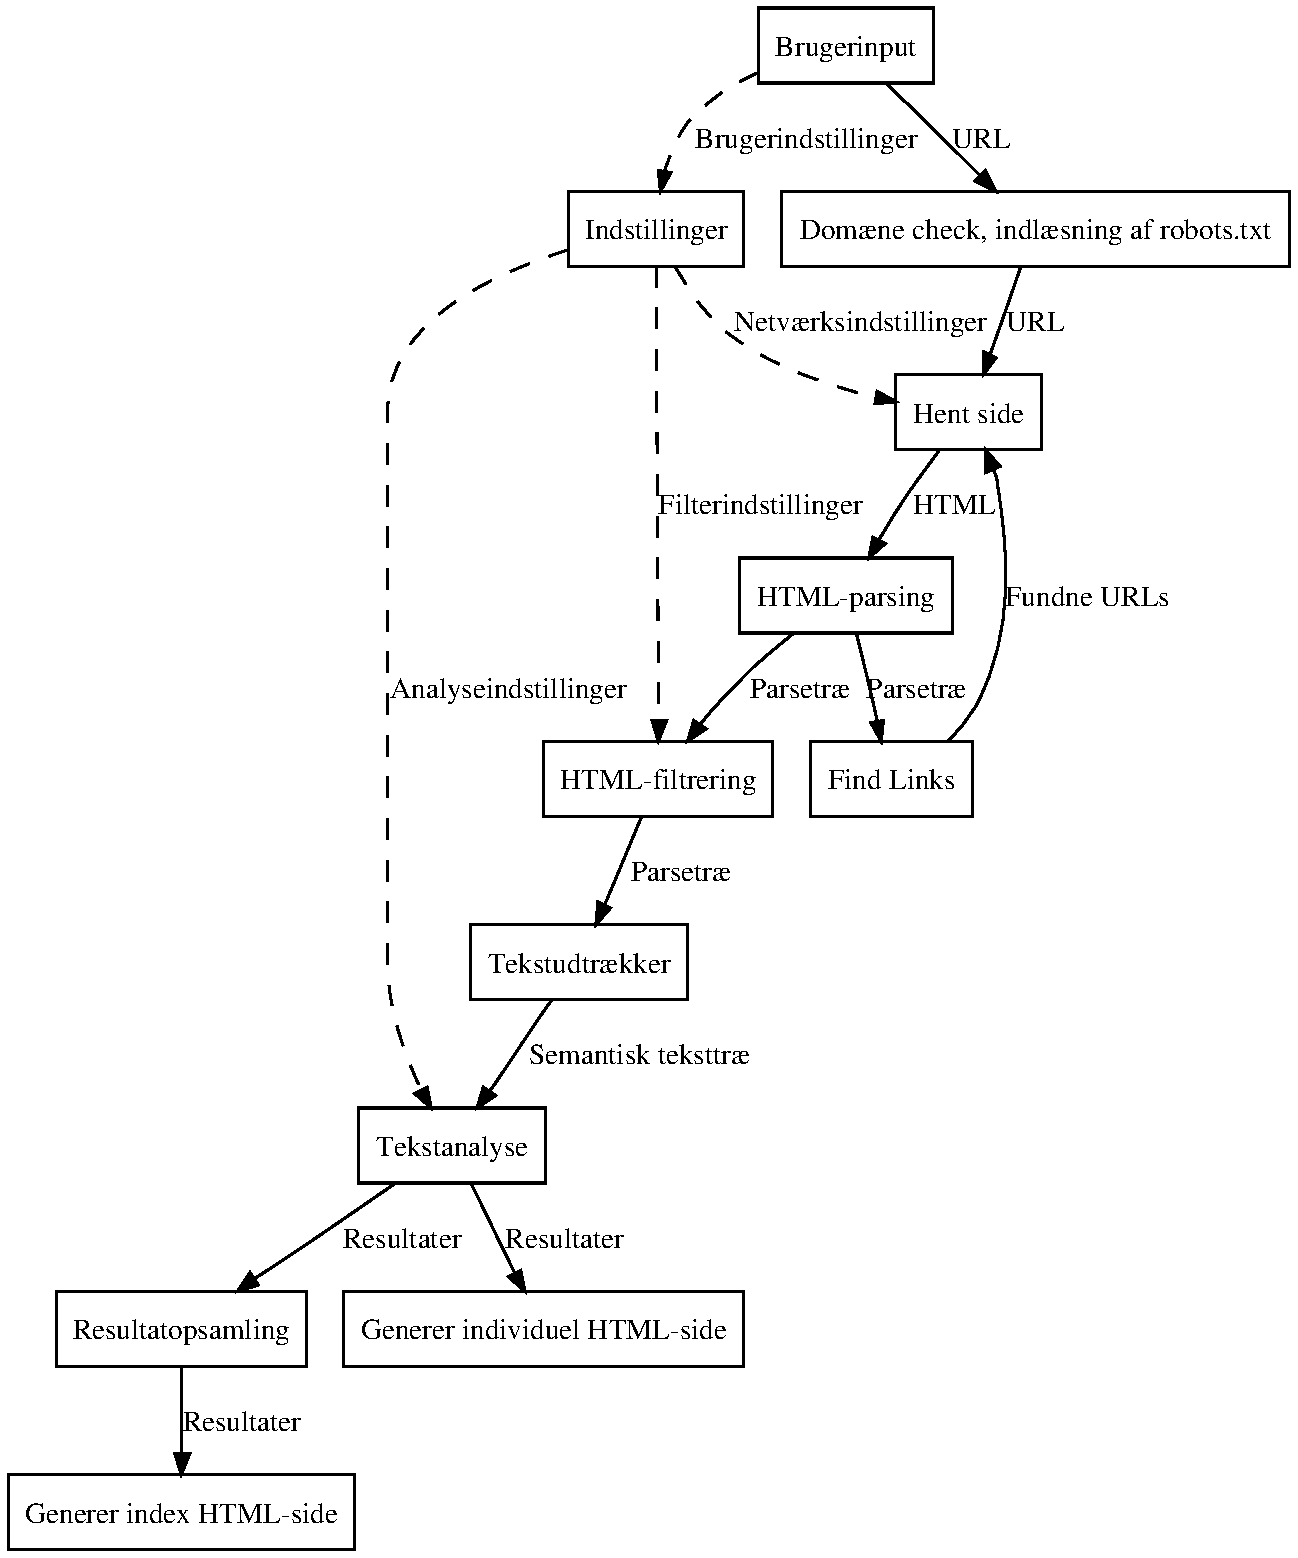
\includegraphics[width=0.55\textwidth]{endeligtdesignill.pdf}
    \caption{Dataflow--diagram}
  \end{figure}
\end{frame}

\subsection{HTML--Parsing}
\begin{frame}[fragile]
  \frametitle{HTML--Parsing}

  \begin{columns}[t]
    \column{.4\textwidth}
    \begin{figure}
\begin{lstlisting}[language=HTML, basicstyle=\tiny\ttfamily,
                   escapechar=\@]
<HTML>
  <HEAD>
    <TITLE>Sidetitel</TITLE>
  </HEAD>
  <!-- En kommentar -->
  <BODY>
    <P>Et afsnit med adskillige s@\ae@tninger.
      Dette er 'den anden s@\ae@tning'.</P>
    <BLOCKQUOTE lang="en">
      <A href="http://en.wikipedia.org/wiki/Hovercraft">
      My hovercraft</A> is full of eels!</BLOCKQUOTE>
  </BODY>
</HTML>
\end{lstlisting}

      \caption{HTML--dokument}
    \end{figure}

\pause

    \column{.6\textwidth}
    \begin{figure}
      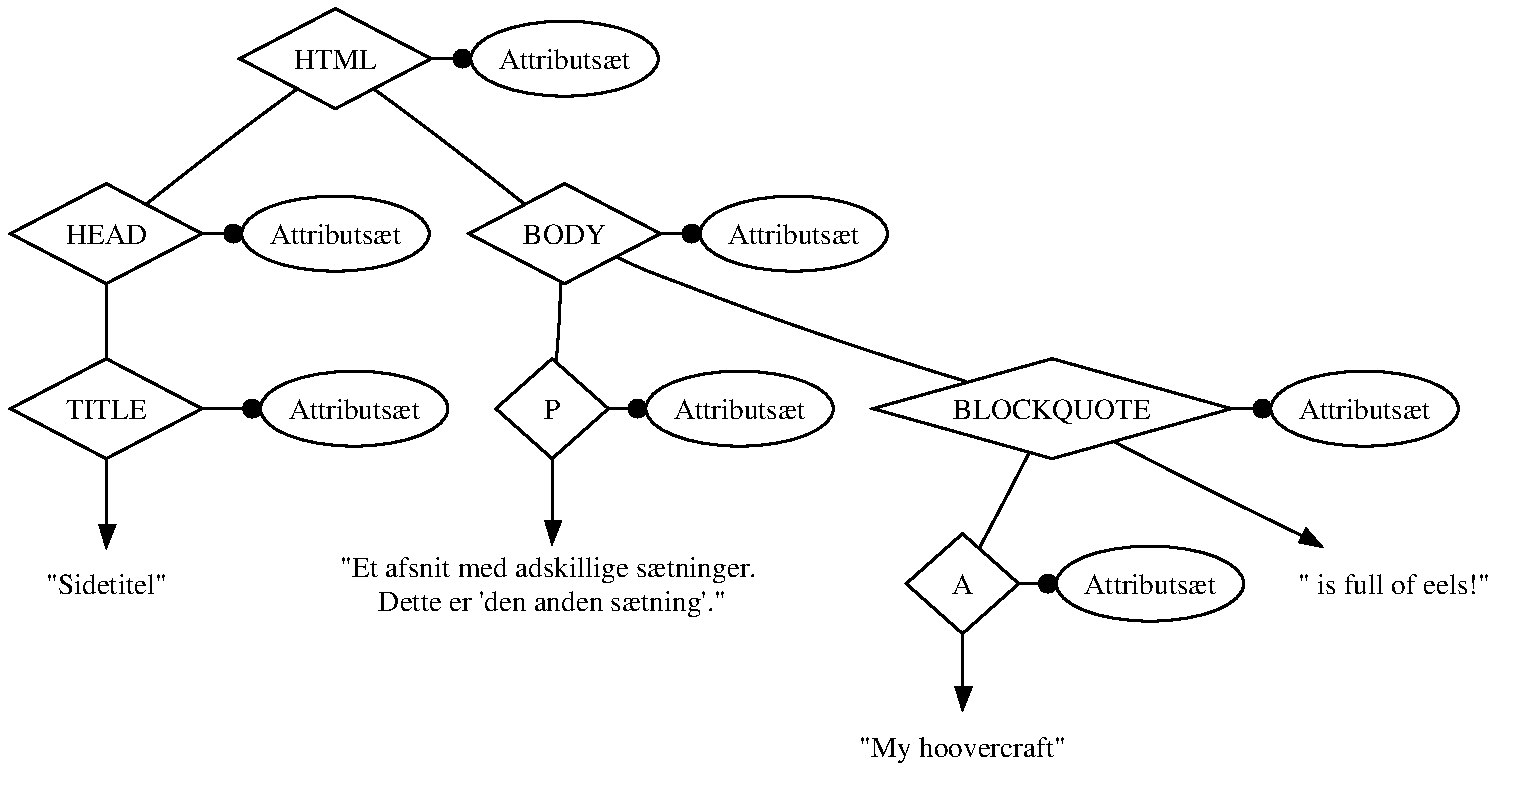
\includegraphics[width=\textwidth]{parsetree.pdf}
      \caption{Parsetræ}
    \end{figure}

  \end{columns}
\end{frame}


\begin{frame}
  \frametitle{Dokument struktur}

  \begin{columns}[t]
    \column{.5\textwidth}
    \begin{figure}
      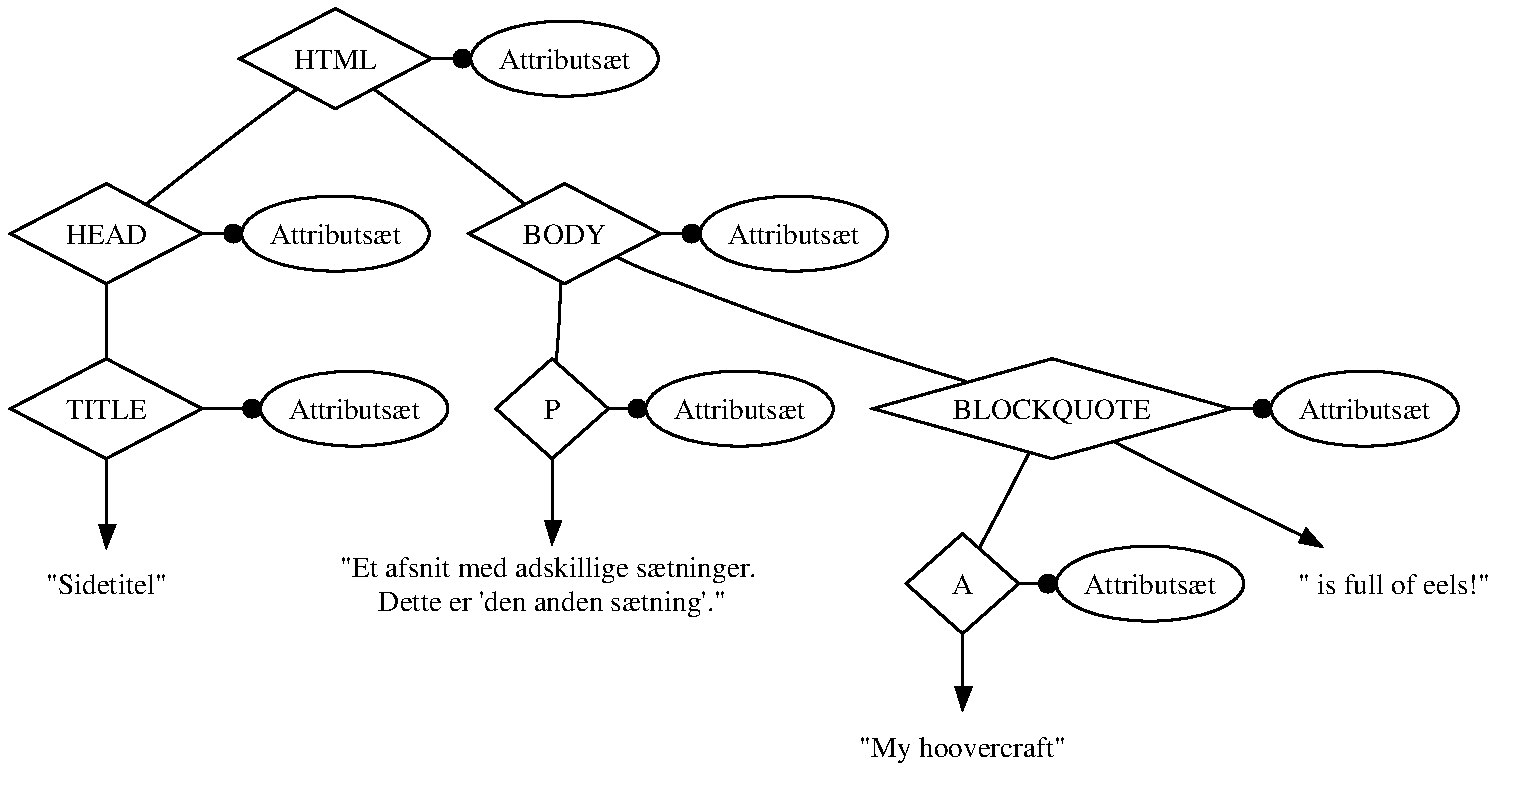
\includegraphics[width=\textwidth]{parsetree.pdf}
      \caption{Parsetræ}
    \end{figure}

    \pause

    \column{.5\textwidth}
    \begin{figure}
      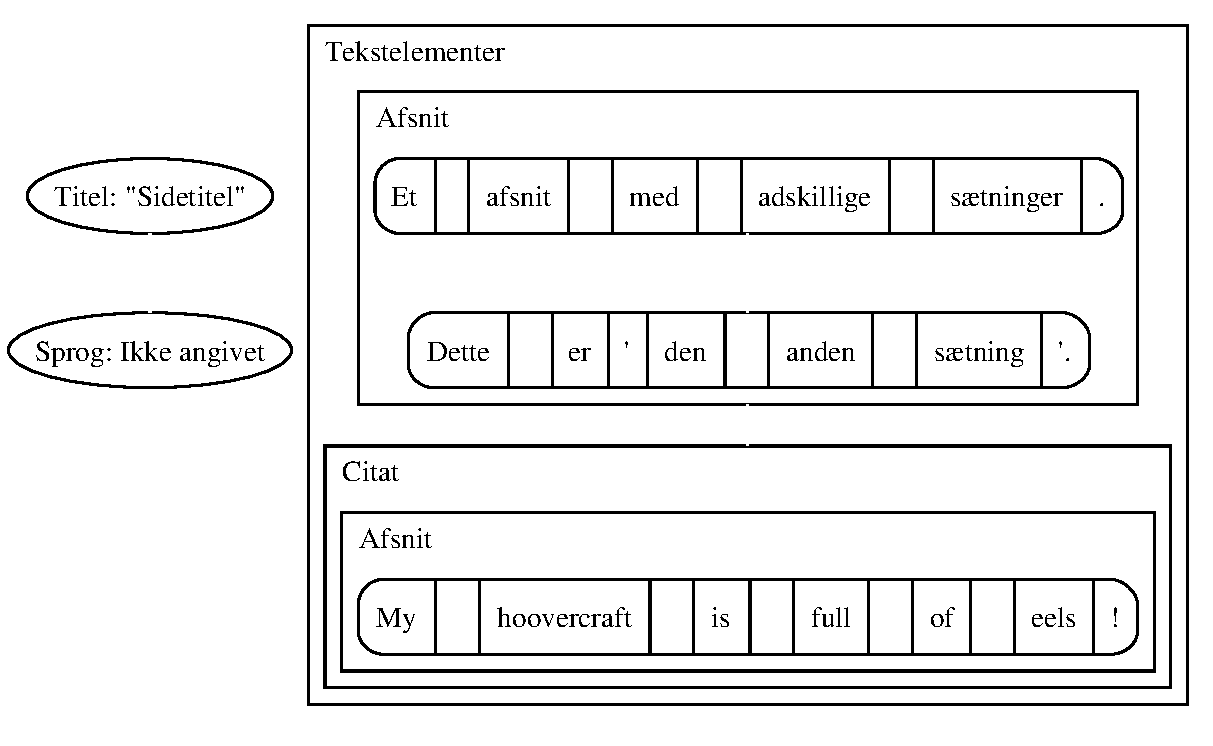
\includegraphics[width=\textwidth]{documentill.pdf}
      \caption{Dokument--struktur}
    \end{figure}
  \end{columns}
\end{frame}

\begin{frame}
  \frametitle{What's Still To Do?}
  \begin{block}{Answered Questions}
    How many primes are there?
  \end{block}
  \pause
  \begin{block}{Open Questions}
    Is every even number the sum of two primes?
  \end{block}
\end{frame}

\begin{frame}
  \frametitle{What's Still To Do?}
  \begin{columns}[t]
    \column{.5\textwidth}
      \begin{block}{Answered Questions}
        How many primes are there?
      \end{block}
      \pause
    \column{.5\textwidth}
      \begin{block}{Open Questions}
        Is every even number the sum of two primes?
      \end{block}
  \end{columns}
\end{frame}


\end{document}
